% !TEX root = main.tex

%%%%%%%%%%%%%%%%%%%%%%%%%%%%%%%%%%%%%%%%%%%%%%%%%%%%%%%%%%%%%%%%%%%%%%%%%%%%%%%%%%%%%%%%%%%%%%%%
\section{結果}
%%%%%%%%%%%%%%%%%%%%%%%%%%%%%%%%%%%%%%%%%%%%%%%%%%%%%%%%%%%%%%%%%%%%%%%%%%%%%%%%%%%%%%%%%%%%%%%%

\subsection{実験課題1}
パルス電源を流した際の電圧波形を図2に示す.
周期 $T$ は $T=400\,[\si{\mu s}]$と測定される.
よって,
$$
L=\frac{(400\times10^{-6})^2}{4\pi^2\times12\times10^{-6}}\fallingdotseq 338\,[\mu H]
$$
と求められる.
\begin{figure}[H]
    \begin{center}
        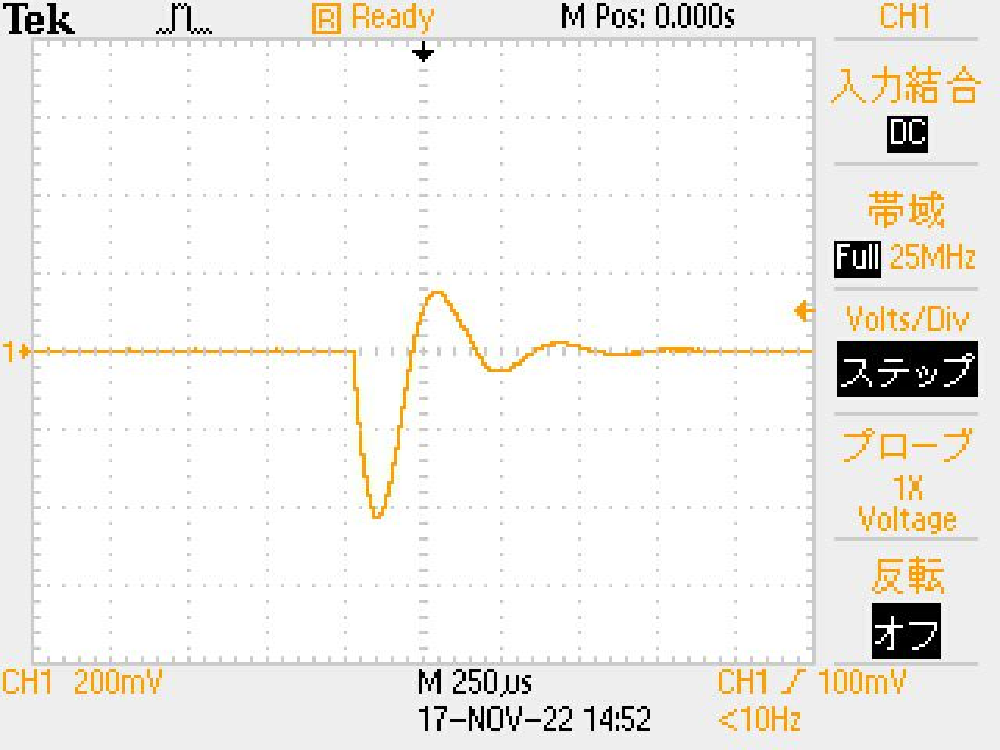
\includegraphics[scale=0.5]{figure2.pdf}
        \caption{セメント抵抗$(1\Omega)$の両端にかかる電圧波形}
    \end{center}
\end{figure}
\newpage

\subsection{実験課題2}
実験課題から算出したインダクタンス$L$の値を用いると,抵抗値$R$は
$$
R=\sqrt[]{\frac{4\times 337.7\times10^{-6}}{12\times10^{-6}}}\fallingdotseq 10.6\,[\Omega]
$$
と求められる.さらに,可変抵抗を調整し,実際に抵抗$R$を回路に接続すると図3に示す
ように電流波形が臨界制動波形となる結果を得られた.
\begin{figure}[H]
    \begin{center}
        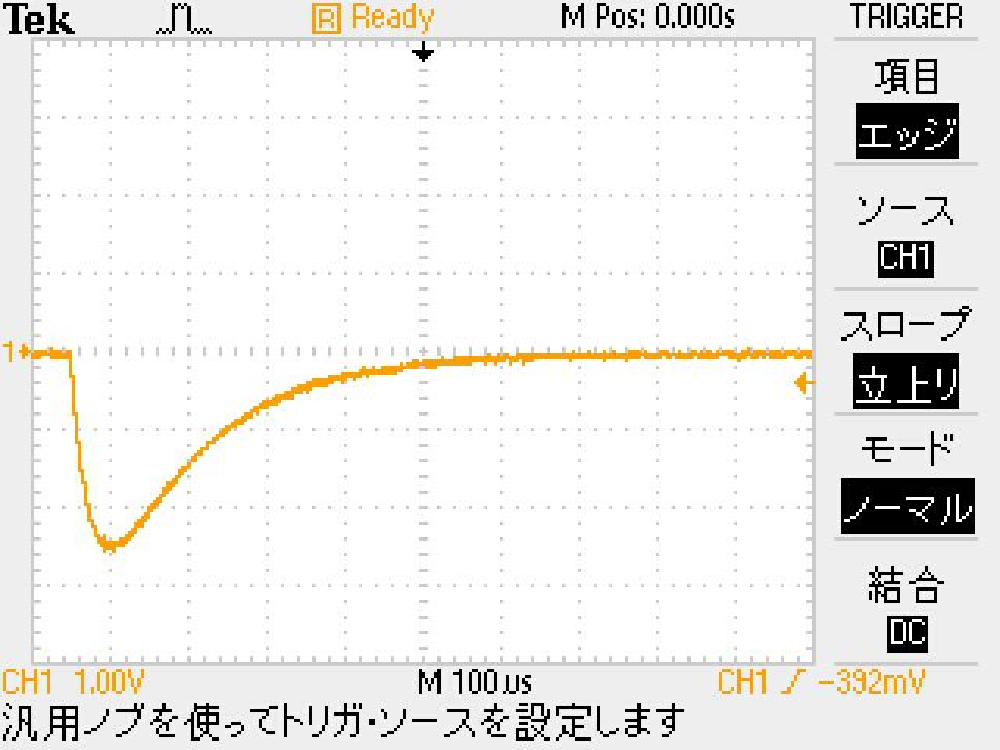
\includegraphics[scale=0.5]{figure3.pdf}
        \caption{臨界制動波形}
    \end{center}
\end{figure}